\documentclass{beamer-control}
\usepackage{beamer-control-singlefile}
\INCLUDEONLY{The Root-Locus Method}
\begin{document}
\CONCEPT{The Root-Locus Method}

\begin{SUMMARY}
\begin{itemize}
\item The root-locus
\item Examples
\end{itemize}
\vfill References:
\begin{itemize}
\item \astrom{§12.5}
\end{itemize}
\end{SUMMARY}



\SUBCONCEPT{The root-locus}

\begin{frame}{Investigating the effects of control}
\begin{itemize}
\item For design methods such as eigenvalue assignment, the complexity of the controller matches the complexity of the process
\item PID instead uses a low number of parameters to control potentially highly complex systems
\item The root-locus method allows us to investigate the effect of a single controller parameter
\item The \textit{root-locus} is a graph of the roots of the characteristic polynomial as a function of the controller parameter
\item This gives us insight into how changes in the parameter influence the system dynamics
\end{itemize}
\end{frame}

\begin{frame}{The method}
\begin{itemize}
	\item Consider a process with transfer function
	\begin{align*}
		P(s) &= \frac{b(s)}{a(s)} = \frac{b_0s^m+b_1s^{m-1}+\cdots + b_m}{s^n+a_1s^{n-1}+\cdots + a_n} \\
		&= b_0\frac{(s-z_1)(s-z_2)\cdots (s-z_m)}{(s-p_1)(s-p_2)\cdots(s-p_n)}
	\end{align*}
	\item Assume the pole excess $n_{pe}=n-m$ is nonnegative
	\item The controller for the system is assumed to be a proportional controller (for simplicity) with transfer function $C(s)=k$
		\item The closed loop characteristic polynomial is 
\[a_{cl}(s)=a(s)+kb(s)\]
and the closed loop poles are the roots of $a_{cl}(s)$
\item The root locus is a graph of the roots of $a_{cl}(s)$ as $k$ varies from $0$ to $\infty$
\end{itemize}
\end{frame}


\begin{frame}{Small $k$}
	\begin{itemize}
		\item Since $a_{cl}(s)$ is of degree $n$, the plot will have $n$ branches
		\item When $k=0$, the closed loop poles are equal to the open loop poles
		\item When there are open loop poles at $s=p_l$ with multiplicity $m$, the characteristic equation is 
		\[(s-p_l)^m\tilde{a}(s) + kb(s)\approx (s-p_l)^m\tilde{a}(p_l)+kb(p_l)=0\]
		where $\tilde{a}(s)$ is the polynomial $a(s)$ with poles at $s=p_l$ factored out
		\item For small $k$, the roots of this equation are given by 
		\[s=p_l + \sqrt[m]{-kb(p_l)/\tilde{a}(p_l)}\]
		\item The root locus will have a star pattern with $m$ branches emanating from the open loop pole $s=p_l$, with angles between branches $2\pi/m$
	\end{itemize}
\end{frame}

\begin{frame}{Large $k$}
	\begin{itemize}
		\item For large gain values we may approximate the characteristic polynomial as
		\[a_{cl}(s) = b(s)\left(\frac{a(s)}{b(s)}+k \right) \approx b(s)\left(\frac{s^{n_{pe}}}{b_0}+k \right)\]
		\item Therefore, for large $k$, the closed loop poles are approximately the roots of $b(s)$ and $\sqrt[n_{pe}]{-b_0k}$
		\item The asymptotes are $n_{pe}$ lines emanating from the centre of mass of poles and zeros
		\item When $b_0k>0$, the lines have angles $(\pi+2l\pi)/n_{pe}$ for $l=1,\cdots,n_{pe}$ with respect to the real line
	\end{itemize}
\end{frame}

\begin{frame}{Summary}
\begin{itemize}
	\item The root locus plot with loop gain as the varied parameter has $n$ branches that start at the open loop poles and end either at the open loop zeros, or at infinity
	\item Open loop poles with multiplicity $m$ will create $m$ branches emanating from the open loop pole
	\item The branches that end at infinity have star-patterned asymptotes
	
\end{itemize}
\end{frame}

\SUBCONCEPT{Examples}

\begin{frame}{Some root loci}
\begin{itemize}
\item Consider the transfer functions
\[P_a(s)=k\frac{s+1}{s^2}, \quad P_b(s) = k\frac{s+1}{s(s+2)(s^2+2s+4)},\]
\[P_c(s) = k\frac{s+1}{s(s^2+1)}, \quad P_d(s) = k\frac{s^2+2s+2}{s(s^2+1)}\]
\end{itemize}
\begin{figure}
	\centering
	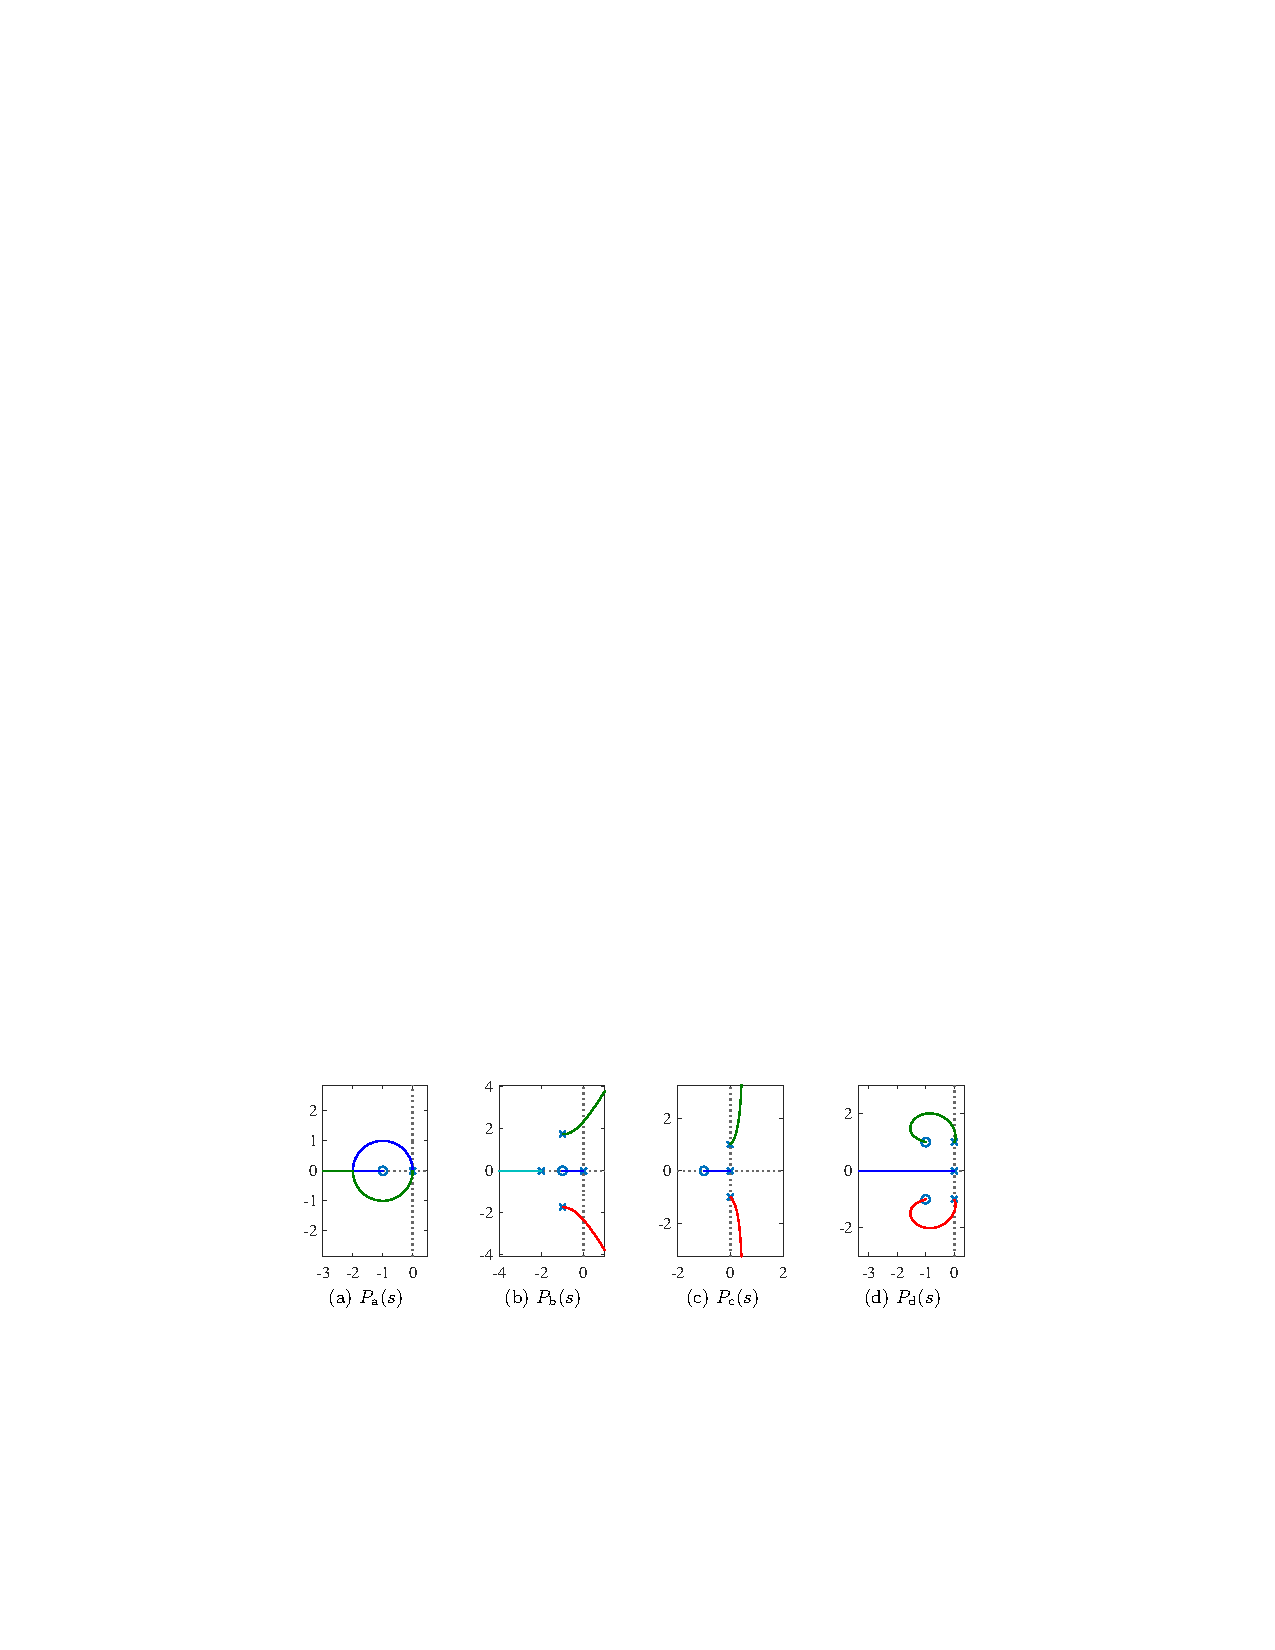
\includegraphics[width=10cm]{figure12.18}\\
	\vspace{-0.2cm}
	\textbf{Figure 12.18:} Examples of root loci.
\end{figure}
\end{frame}

\begin{frame}{Root locus for design}
\begin{itemize}
	\item Consider the previously defined transfer function $P_c(s)$ as a representation of PI control of a system with
	\[P(s)=\frac{1}{s^2+1}, \quad C(s)=k\frac{s+2}{s}\]
	\item From the root locus of $P_c(s)$, the system is unstable for all gain values and hence cannot be stabilised by PI control
	\item PID control may be implemented by using the controller
	\[C(s)=k\frac{s^2+2s+2}{s}\]
	whcih gives the transfer function $P_d(s)$
	\item This system is stable and we can choose $k$ to place the poles in desirable locations
\end{itemize}
\end{frame}

\SUMMARYFRAME
\FINALE

\end{document}
